\documentclass[12pt]{article}
\usepackage{graphicx}
\graphicspath{{Images/}}
\usepackage{textcomp} %for the copywrite symbol
%\linespread{1.6} %sets lines to 1.5 spacing.  1.6 would be double spaced
\usepackage[margin=1.0in]{geometry}
\usepackage[semicolon,round,sort&compress,sectionbib,numbers]{natbib}  
\usepackage{chapterbib}  
\usepackage{amsmath}
\usepackage{subcaption}
\usepackage{appendix} %for appendices
\usepackage{float}
\usepackage{listings}

\usepackage{hyperref} %make stuff clickable
\hypersetup{
	colorlinks,
	citecolor=black,
	filecolor=black,
	linkcolor=black,
	urlcolor=black
}


\usepackage{physics}  %for bras and kets!
\newcommand{\angstrom}{\mbox{\normalfont\AA }} %makes \angstrom do its thing!

\title{Lithium ELNES with WIEN2k}

\begin{document}
\maketitle

\tableofcontents

\section{Tools}	
Here's a list of software I use to run simulations.  I've put some installation instructions for linux as needed.  

\begin{itemize}
	\item Wien2k  - If you are reading this guide, you either already have it installed somewhere, or should figure out how to do that before buying a license.  
	
	\item  VESTA: \url{http://jp-minerals.org/vesta/en/download.html}.  Download the .rpm file, install it with your package manager, eg. ``sudo apt-get vesta...rpm"
	
	\item Critic2: \url{https://github.com/aoterodelaroza/critic2}.  Download the zip from GitHub, unzip where you want to install it eg $\sim$/Programs or something), install (using dnf/apt-get) autoconf, automake, and your favourite flavour of fortran.  Then run the 4 commands from the readme: ``autoreconf -i", ``./configure", ``make", and ``(sudo) make install".   You may or may not need the sudo for the last one. 
	
\end{itemize}
	
\section{Setup}	

We need a couple things to get started for ELNES simulations.  Foremost is a crystal structure.  You can either get this from the literature, XRD, or alternatively Materials Project: \url{https://materialsproject.org/}.  Download a cif (the primative cell typically) or enter the coordinates directly into the wien2k struct gen tool.  

Make a new Wien2k session: 
\begin{figure}[H]
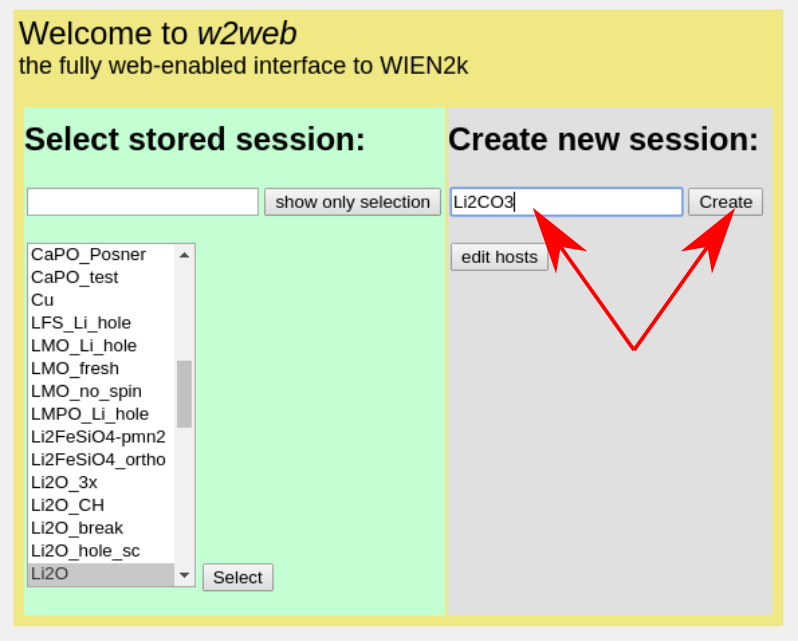
\includegraphics[scale=0.3]{./images/new_session.png}
\end{figure}

Create/change a working directory, and change the session information for parallel calculation.
	
	\begin{figure}[H]
		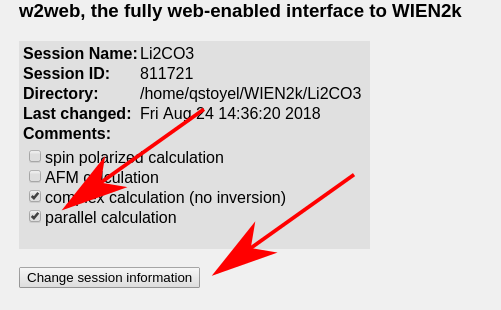
\includegraphics[scale=0.5]{./images/parallel.png}
	\end{figure}
	
You will also need to make a ``.machines" file which you can either steal from one of my directories, look in the user guide and make your own, cut and paste the one from below, or wait for w2web to automatically generate one at some point after it inevitably crashes on something.
Sample .machines file: 

\begin{lstlisting}
#=======================================
#This is a valid .machines file
#
granularity:1
1:localhost #as many of these lines as you want cpu cores running
1:localhost
1:localhost
1:localhost
1:localhost
1:localhost

\end{lstlisting}

Next, go make a struct file, with struct gen, either by importing the cif, or entering the positions manually.  Use VESTA (drag n' drop the .struct file) to make sure that the structure is what you'd expect. 
In our Li2CO3 case this looks like: 

	\begin{figure}[H]
	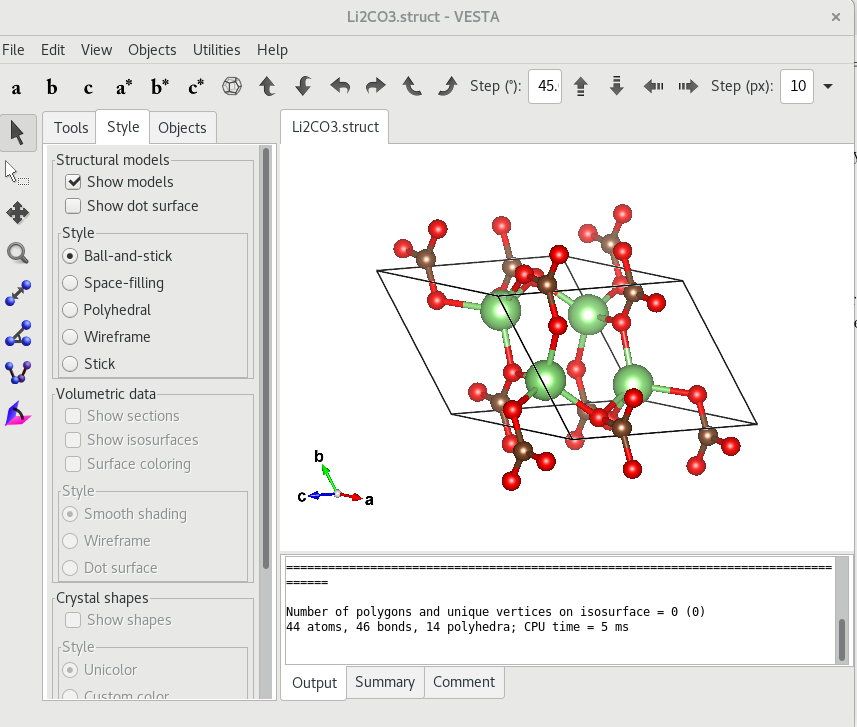
\includegraphics[scale=0.4]{./images/Li2CO3_struct.png}
\end{figure}


Now we need to initialize the case.  You can do this in w2web, but we are going to get our hands dirty anyways, so I like to use the command line for this and see what's actually going on.  Run ``init\_lapw" in the case directory.

\begin{itemize}
	\item \textbf{setrmt}. Sets the muffin tin size on the atoms.  Reduce the sphere size by 0\% using either old or new scheme and accept, it doesn't matter much as we are going to change this all later.
	\item  \textbf{nn}.  Checks for overlapping muffin tins. Enter ``2.0", close the first file and use the new NN file if it suggests it, run nn with 2.0 again, look at how much ``wiggle room" you have on the spheres, see pic. 
	
	\begin{figure}[H]
		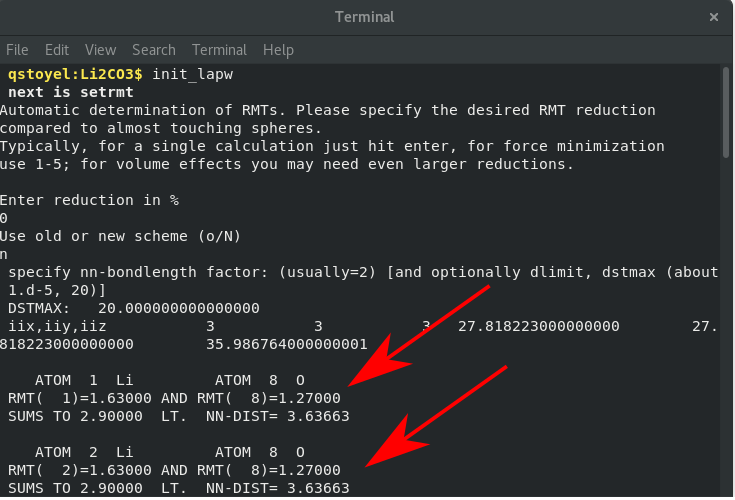
\includegraphics[scale=0.4]{./images/init_lapw2.png}
	\end{figure}
	
	\item \textbf{sgroup}. Verifies the space group.  Again, accept any changes the program makes, these steps are all about reducing the cell symmetries to what they should be. Again, the files can be largely  ignored at this point, with the exception of indication of a Bravais lattice change, in which case just take the new struct file. If so, nn and sgroup will run again with ``nice" results.  
	\item  \textbf{symmery}. Generates all the symmetry operations. Run it and continue (enter ``c")
	\item  \textbf{lstart}. Set spin state, pick your XC kernel, define cutoff between core and valence states.  Accept default spins (up, the no spin case), unless you have a transition metal. Select GGA PBE as you XC potential, again, unless you have reason to suspect otherwise. Picking the energy is the most important part of this first run init\_lapw, we want to try to get the Li 1s states to be treated as core states.  They typically have energies of $\sim$-3.7Ry, so try with -3.5Ry to make sure they will be treated as core states and look in case.outputst (the file that pops up), for the following lines for the lithium atom and look at the 1S states:  
	
	\begin{lstlisting}
          E-up(Ry)      E-dn(Ry)   Occupancy   q/sphere  core-state
1S      -3.801947     -3.785288  1.00  1.00    0.9859  T
1S      -3.801947     -3.785288  1.00  1.00    0.9859  T
2S      -0.236699     -0.003313  1.00  0.00    0.0468  F
2S      -0.236699     -0.003313  1.00  0.00    0.0468  F
	\end{lstlisting}
	
	These indicate the core states (T/F), their energy levels (in this case $\sim$ -3.8eV) and how much the electrons in these states live in the muffin tins (0.9859).  As this is less than 1, it means a lot of 1S lithium electron is leaking out of the muffin tins, which is why there should now be all kinds of warnings popping up.  So go ahead and ``ctrl-c" out of init\_lapw.
	
\end{itemize}  

To fix the leakage problem, the Lithium muffin tins must be bigger.Ideally they should be just big enough to hold all of the 1S electrons, without making them too different from the other muffin tins, as the larger this difference, the harder things get to calculate/converge.  In this case, try Li=1.8,  C=1.2, O=1.22 and try init\_lapw again, if that still didn't work (lstart still had leakage errors), keep going until it does, in this case RMT's of Li=2.0,  C=1.14, O=1.22.  At this point you should be able to run through init\_lapw quite quickly.  Go through it one last time in full to make sure everything is set correctly: 

\begin{itemize}
	\item \textbf{setrmt}: Setrmt will try to reset the muffin tins to the defaults, make sure to discard these (enter d)
	\item \textbf{nn} Make sure you don't get errors, and that everything is as tight as it can be, in this case the Oxygen-carbon spacing is the limiting factor.  
	\item \textbf{sgroup} Should run fine.
	\item  \textbf{symmery} Should run fine. 
	\item \textbf{lstart} Now that the lithium 1S states are well contained, cre states can be selected based on containment instead of energy meaning, the higher energy states (2S, P) of other elements can still be treated as valence.  Entering 0.995 should be sufficient here, but make sure to verify that the lithium states are still core states.
	\item \textbf{kgen} Set the RkMax value in case.in1\_st:		
	\begin{figure}[H]
		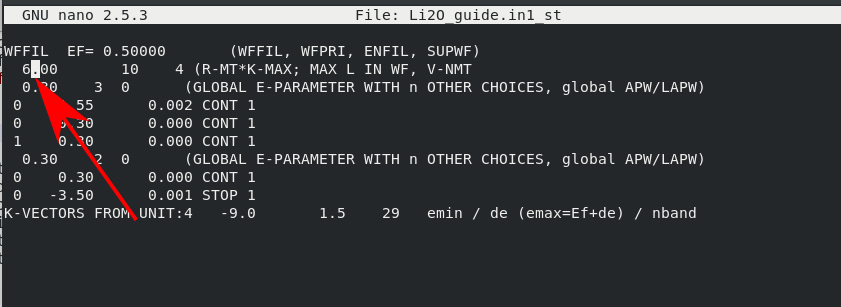
\includegraphics[scale=0.4]{./images/init_lapw3.png}
	\end{figure}
	and then pick a k\_point number.  Both of these values should initially be taken for fast convergence, in this case I chose RkMax=7.0, and 8 k points (Li2CO3 is an insulator, for metals 1000 k points is a good starting point).
	\item \textbf{Dstart}: make sure to pick non spin polarized, unless you have reason to believe otherwise (is there a transition metal in your sample?)
\end{itemize}

Assuming tere were no warnings in the final run through init\_lapw, we can now start convergence.

\section{Convergence}
Ideally, you want to converge everything regarding your simulation.  Typically this is cell parameters, k points and Rkmax.  The first step is to just make sure the calculation converges, running it with a small RKmax and few kpoints and making sure it finishes.  

\subsection{Cell parameters:}
This process works best from W2Web, as described in the tutorials and the muffin tins from setrmt reduced by a healthy percentage ($\sim$ 5-10\%) to avoid nn errors.   As  a number (5-11+) of calculations are run in this process, a low number of k points and RKMax values is ideal here. For Li2CO3, I used 16 kpoints and an RKmax of 7.   In the x ``optimize" tab, choose what you want to optimize, the first option (volume) works well, unless you have suspicions otherwise.  Enter a range of values of test volumes, see picture:

\begin{figure}[H]

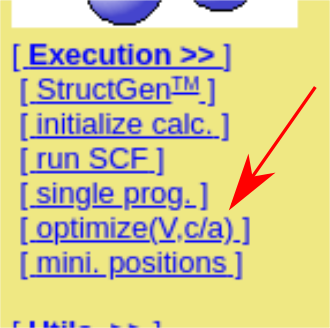
\includegraphics[scale=0.3]{./images/vol_opt_menu.png}
~
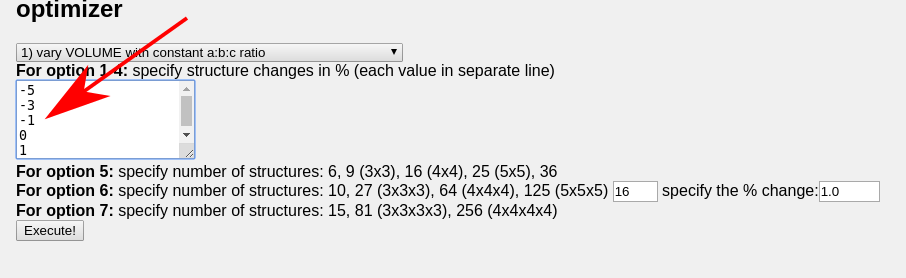
\includegraphics[scale=0.3]{./images/vol_opt.png}



\end{figure}


Also make sure to edit ``optimize.job" to enable parallization by moving the ``\#" to after the ``-p" in the run\_lapw line: 

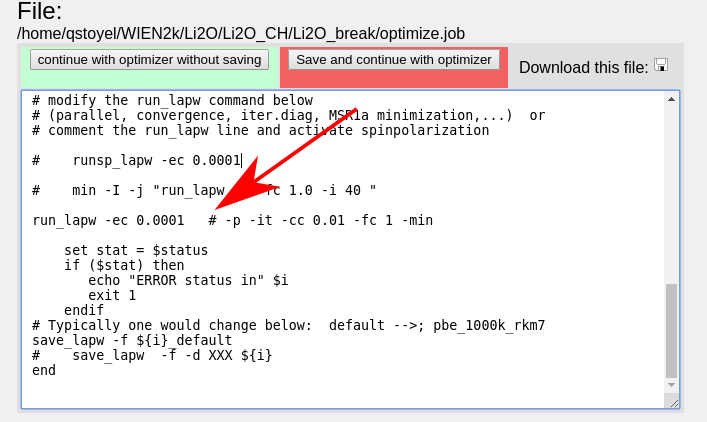
\includegraphics[scale=0.4]{./images/vol_opt2.png}

You can then ``run optimize.job" from w2web. This job is okay to run in the background, so you can close the browser and run it overnight as well.  When it is done, plot the ``Energy vs Volume," which should give you something like this:\\
  
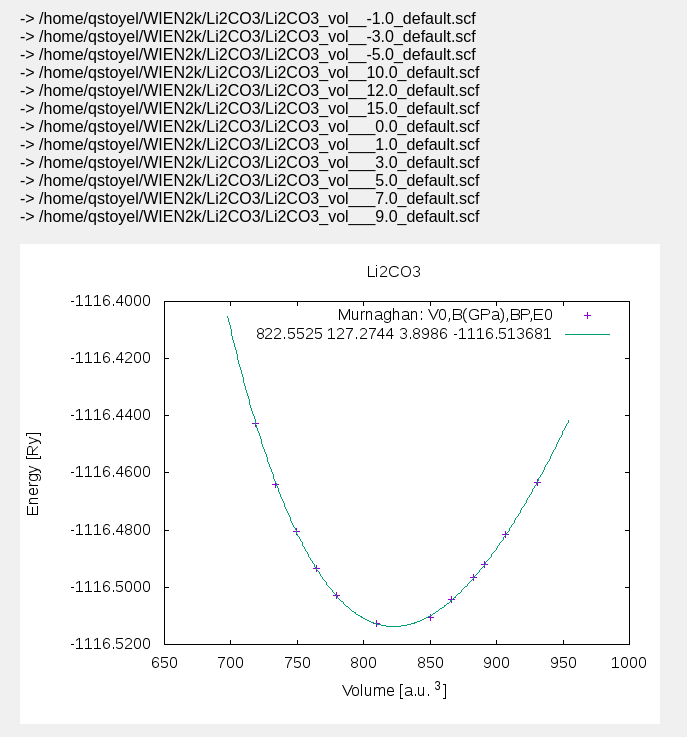
\includegraphics[scale=0.3]{./images/E_vs_V.png}

In the case of Li2CO3 and the original cif from materials project, quite a range of volume options were needed to locate the minimum.  The graph indicates that a 3-4\% increase should correspond to the optimized structure.  To use this structure, search the case directory for all the struct files and rename the appropriate one to case.struct, for Li2CO3 this was ``Li2CO3\_vol\_\_\_3.0.struct $\to$ Li2CO3.struct". Alternatively, cut and paste the lattice parameters from this file into the w2web structgen tool.    Finally, rerun init\_lapw and readjust sphere sizes as necessary to account for the increase (or decrease) in cell size. 

\subsection{K point and RKMax convergence}

To converge these parameters, again start with very low values and then increase them, checking the total energy to determine when they are converged.  Generally k points are easier to converge, so start with them and then move on to RKMax. The procedure for converging both of these values is:

\begin{itemize}
	\item set/increase kpoints or RKMax, either by re-running ``x kgen" or editing case.in1 and case.in1\_st.
	
	\item Run the scf cycle using ``run\_lapw -p -NI", the NI flag means it will continue from where the previous calculation left off which saves time. I would still run your final choice from scratch though.
	
	\item Check the energy in case.scf.  To do this, find it in ``scf files" on w2web and use ctrl+f in your browser to search the file for ``:ene" , which should appear in a line that looks like: 
	
		\begin{lstlisting}
:ENE  : ********** TOTAL ENERGY IN Ry =        -1116.50733157
		\end{lstlisting}
	
	There will be one of these lines for each scf cycle, so find the last one in the document and note the energy. 
	
	
	\item loop through the first 3 steps until the energy no longer changes significantly when you increase the kpoints/RKMax.  A table is useful here to track these effects:
	
\end{itemize}

\begin{table}[H]
	\centering
\begin{tabular}{ccc}

			kpoints & RKMax & Energy \\
			\hline
			8 & 7.0 &  -1116.5073\\
			16 & 7.0 & -1116.4971\\
			32 & 7.0 & -1116.4975\\
			32 & 8.0 & -1116.5038\\
			32 & 9.0 & -1116.5045\\
			
			

\end{tabular}

\end{table}


\section{TELNES3}

Once the calculation is converged, ELNES can be calculated.  Again, there is a large list of parameters that must be set for in order to obtain reasonable results. It is also worth converging Kpoints and RKMax against the spectra as well.\\
The majority of the important parameters need to be set in the \textbf{case.innes} file, which is easiest through w2web.  Choose the right atom (in this case Li1) for the edge, and the right atomic numbers:  

\begin{table}[H]
	\centering
	\begin{tabular}{ccc}
		
		Edge & n & l \\
		\hline
		K & 1 &0 \\
		L1 & 2 & 0 \\
		L23 & 2 &1\\
		M45 & 3 & 2\\
	\end{tabular}
	
\end{table}

Next, set the edge onset,edge values can be found at \url{http://www.kayelaby.npl.co.uk/atomic_and_nuclear_physics/4_2/4_2_1.html} as well as at a number of other locations.  Set the beam energy to it's correct value, same goes for the collection and convergence angles, although TELNES is relatively robust to these: eg 5mrad produces very similar results to 1 mrad.\\

Set the energy grid to a large range of values, eg -20-50eV so you can see all of the features that might appear.  The defaults for the remaining values should be fine.\\

In addition to the case.innes parameters, increase the number of kpoints, to at least double, or 10$\times$, so that there is less doubt about this being converged, use x kgen for this.  \\

Increase the upper energy limit in case.in1 from 1.5 to $\sim$ 2-3.5, see picture.  This value defines how many higher energy states are included in Ry (1 Ry $\approx$13.6 eV, 1.5Ry $\approx$ 20eV). Therefore, to obtain the correct ELNES for features more than 20eV from the onset,  this should be increased.  \\

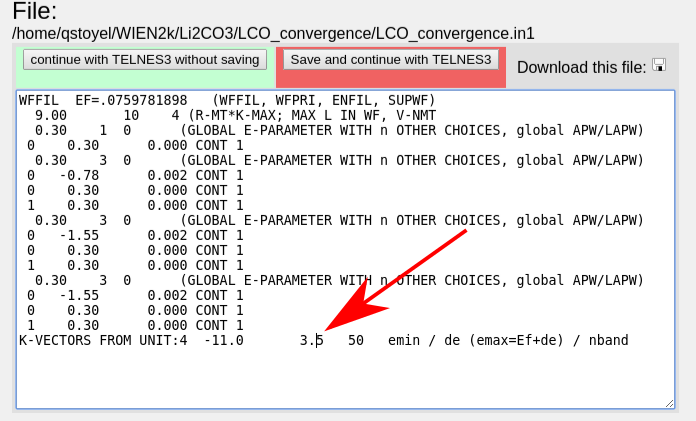
\includegraphics[scale=0.4]{./images/in1_edit.png}


\section{Common Errors Thrown by Code}

\subsection{NN in Optimization}
Crashes the first scf cycle almost immediately, due to overlapping muffin tins resulting from a decreased cell size.  Solution: decrease all muffin tin sizes before running ``x optimize".


\subsection{GMax Value less than Gmin}

Occurs in \textbf{dstart}, fix is to bump up the Gmax value in case.in2 from 12.00 to 14.00 or 16.00.

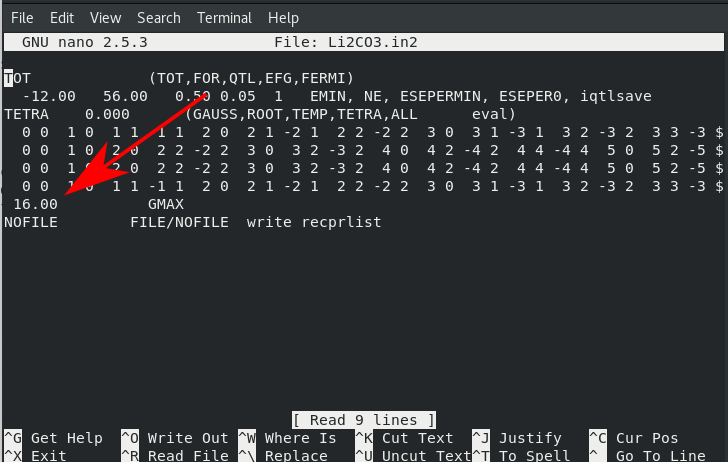
\includegraphics[scale=0.5]{./images/gmax_err.png}



\begin{itemize}
	\item \textbf{setrmt}
	\item \textbf{nn}
	\item \textbf{sgroup}
	\item  \textbf{symmery}
	\item \textbf{lstart}
	
\end{itemize}


\end{document}